% !TEX root = monografia.tex
\chapter{Aprendizado de Reforço}
\label{cap:reforco}

\begin{figure}
    \centering
        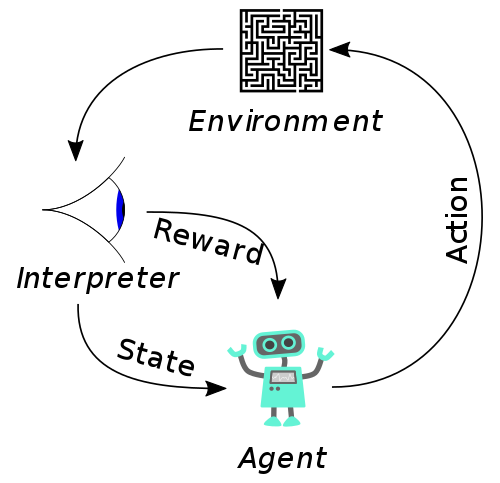
\includegraphics[width=5cm]{figuras/rl}
    \caption{Ilustração de Aprendizado de Reforço}
    \label{fig:rl}
\end{figure}

Aprendizado de Reforço (AR) é uma das grandes áreas que compõe Aprendizado de Máquina (?),
onde são estudados algoritmos que descrevem o comportamento de \textit{agentes} em um \textit{ambiente},
buscando o maior \textit{retorno} por suas ações (ilustrado na figura~\ref{fig:rl}).

Essa definição geral admite aplicação em uma grande quantidade de problemas (?),
sendo limitada principalmente pela existência de um ambiente que possa ser eficientemente simulado durante o processo de aprendizado do algoritmo.
Consequentemente, o aprendizado muitas vezes depende de uma quantidade grande de recursos computacionais.

Geralmente, os problemas da área são formulados como Processos de Decisão de Markov (MDP) finitos(?).
Um Processo de Decisão de Markov é uma quíntupla $(S,A,T,R,\gamma)$(?), onde:
\begin{itemize}
    \item $S$ é o conjunto de estados (que representa o ambiente)
    \item $A$ é o conjunto de ações que o agente pode tomar
    \item $T: S \times S \times A \to [0, 1]$ representa a probabilidade de um novo estado $s'$ dados o estado atual $s$ e ação $a$
    \item $R: S \times A \to \mathbb{R}$ a função de retorno
    \item $\gamma \in [0, 1]$ é um fator que determina o a importância de retornos futuros comparados com retornos imediatos.   
\end{itemize}

Nesse trabalho, trataremos de um problema de \textit{informação imperfeita},
onde o agente não poderá observar diretamente o estado $s$,
só uma parte dele $o(s)$. 
Além disso, temos um conjunto de estados chamado de \textit{estados terminais},
onde a probabilidade de transição para qualquer outro estado é 0.

O agente define uma \textit{política} $\pi: A \times o(S) \to [0, 1]$ 
que representa a distribuição de probabilidade da escolha de uma ação em um dado estado $\pi(a | o(s))$.

Assim temos um mecanismo para gerar amostras, 
partindo de um estado $S_0$,
selecionamos uma ação $A_0 \sim \pi(a | o(S_0))$,
deixamos o agente observar $R_1 = R(S_0, A_0)$
e selecionamos um estado $S_1 \sim T(s | S_0, A_0)$,
a partir do qual o processo se repete,
até alcançar um estado $S_T$ que seja terminal.
Ao conjunto 
$S_0, A_0, R_1, S_1, A_1, R_2, S_2, A_2, ..., R_T, S_T$,
damos o nome de \textit{episódio}.

O objetivo dos nossos agentes é, 
através de suas observações dos episódios, 
aprender uma política que maximiza o \textit{retorno descontado} $G_1$ onde:
$G_t := R_t + \gamma R_{t + 1} + \gamma^2R_{t + 2} + ... = R_t + \gamma G_{t + 1}$.

Será útil para nossa discussão definir a função \textit{valor} $v_{\pi}(s) = \mathbb{E}_{\pi}[G_t | S_t = s]$
de um estado $s$, para a política $\pi$ em um tempo $t$ qualquer,
e a função \textit{ação-valor} $q_{\pi}(s, a) = \mathbb{E}_{\pi}[G_t | S_t = s, A_t = a]$.

Isso é porque muitos algoritmos de AR consistem em definir uma política,
estimar a função valor ou ação-valor dessa política, e usá-lá para criar uma nova política,
aumentando a probabilidade de visitar um estado quanto maior for o seu valor (nesse caso, é necessário também modelar o ambiente),
ou aumentando a probabilidade de tomar ações quanto maior for a ação-valor.